% \begin{document}

\chapter{SPSC Lockless Queue}

A single producer single consumer (SPSC) lockless queue is a data exchange queue
between a producer and a consumer. The SPSC lockfree queue enables data exchange
between producer and consumer without the use of a lock, allowing both producer
and consumer to make progress in all scenarios.\newline

An example application of SPSC queue is a data exchange interface between ASIC
and the CPU in a driver implementation.\newline

A real implementation need to account for memory ordering effects specific to
the architecture. For example, ARM has weak memory ordering model where
read/write may appear out-of-order between CPUs. In this chapter we will assume
\textit{logical} execution order where each command is perceived issued
sequentially (even across CPUs) to focus the discussion on describing the system
using TLA+.
\newline

\section{Requirement}

The following describes the SPSC queue requirements: 

\begin{itemize}
    \item Two executing context, reader and writer
    \item Writer advances wtpr after writes
    \item Reader advances rtpr after reads
    \item If rtpr equals wptr, queue is empty
    \item If (wtpr + 1) \% N equals rptr, queue is full
\end{itemize}

The following is an example of a SPSC queue:
\begin{center}
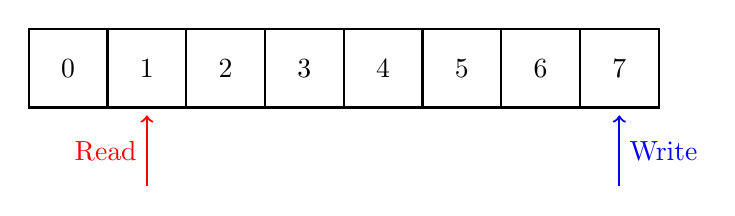
\begin{tikzpicture}
\foreach \i in {0,1,2,3,4,5,6,7} {
    \draw[thick] (\i,0) rectangle (\i+1,1); % Draw each spot in the queue
    \node at (\i+0.5, 0.5) {\i}; % Label each spot
}
\draw[thick, ->, red] (1.5, -1) -- (1.5, -0.1) node[midway, left] {Read};
\draw[thick, ->, blue] (7.5, -1) -- (7.5, -0.1) node[midway, right] {Write};
\end{tikzpicture}
\end{center}

Since reader and writer execute in different context, the instructions in read
and write can interleave in \textit{any} way imaginable:
\begin{itemize}
    \item Reader empty check can happen just as writer is writing data
    \item Writer full check can happen just as reader is reading data
    \item Reading and writing can occur concurrently
\end{itemize}

The key observations is the index held by write pointer is reserved by the
writer. Similarly, index held by the read pointer is reserved by the reader. The
only exception is when read pointer equals to write pointer, then the queue is
empty. Given the possible ways the reader and writer execution can interleave, 
we can use TLA+ to verify the design.

\section{Spec}

TLA+ specification can be writen using its native formal specification language,
or a C-like syntax called PlusCal (which transpiles down to itse native form).
In this example, I chose to implement the specification using PlusCal, since the
content to be verified is psuedo implementation. While it is possible specify
SPSC in native TLA+, I find the approach more error prone as each line is
effectively an individual state to be modeled.\newline

The following is a snippet of the \textit{Spec} written in PlusCal:\newline
\begin{ppcal}
procedure reader()
begin
r_chk_empty:        if rptr = wptr then 
r_early_ret:            return;
                    end if;
r_read_buf:         assert buffer[rptr] # 0;
r_cs:               buffer[rptr] := 0;
r_upd_rtpr:         rptr := (rptr + 1) % N;
                    return;
end procedure; 

procedure writer() 
begin
w_chk_full:         if (wptr + 1) % N = rptr then 
w_early_ret:            return; 
                    end if;
w_write_buf:        assert buffer[wptr] = 0;
w_cs:               buffer[wptr] := wptr + 1000;
w_upd_wptr:         wptr := (wptr + 1) % N;
                    return;
end procedure; 
\end{ppcal}\newline
\begin{tlatex}
\@x{ {\p@procedure} reader ( )}%
\@x{ {\p@begin}}%
 \@x{ r\_chk\_empty\@s{.5}\textrm{:}\@s{3}\@s{28.7} {\p@if} rptr \.{=} wptr
 {\p@then}}%
 \@x{ r\_early\_ret\@s{.5}\textrm{:}\@s{3}\@s{32.8} {\p@return}
 {\p@semicolon}}%
\@x{\@s{32.8} {\p@end} {\p@if} {\p@semicolon}}%
 \@x{ r\_read\_buf\@s{.5}\textrm{:}\@s{3}\@s{32.8} {\p@assert} buffer [ rptr ]
 \.{\neq} 0 {\p@semicolon}}%
 \@x{ r\_cs\@s{.5}\textrm{:}\@s{3}\@s{32.8} buffer [ rptr ] \.{:=} 0
 {\p@semicolon}}%
 \@x{ r\_upd\_rtpr\@s{.5}\textrm{:}\@s{3}\@s{32.8} rptr \.{:=} ( rptr \.{+} 1
 ) \.{\%} N {\p@semicolon}}%
\@x{\@s{32.8} {\p@return} {\p@semicolon}}%
\@x{ {\p@end} {\p@procedure} {\p@semicolon}}%
\@pvspace{8.0pt}%
\@x{ {\p@procedure} writer ( )}%
\@x{ {\p@begin}}%
 \@x{ w\_chk\_full\@s{.5}\textrm{:}\@s{3}\@s{32.8} {\p@if} ( wptr \.{+} 1 )
 \.{\%} N \.{=} rptr {\p@then}}%
 \@x{ w\_early\_ret\@s{.5}\textrm{:}\@s{3}\@s{45.1} {\p@return}
 {\p@semicolon}}%
\@x{\@s{32.8} {\p@end} {\p@if} {\p@semicolon}}%
 \@x{ w\_write\_buf\@s{.5}\textrm{:}\@s{3}\@s{32.8} {\p@assert} buffer [ wptr
 ] \.{=} 0 {\p@semicolon}}%
 \@x{ w\_cs\@s{.5}\textrm{:}\@s{3}\@s{32.8} buffer [ wptr ] \.{:=} wptr \.{+}
 1000 {\p@semicolon}}%
 \@x{ w\_upd\_wptr\@s{.5}\textrm{:}\@s{3}\@s{32.8} wptr \.{:=} ( wptr \.{+} 1
 ) \.{\%} N {\p@semicolon}}%
\@x{\@s{32.8} {\p@return} {\p@semicolon}}%
\@x{ {\p@end} {\p@procedure} {\p@semicolon}}%
\end{tlatex}

Note some lines start with \textit{label} (eg. r\_chk\_empty). All the actions
associated with the label is assumed executed atomically. This is reflected in
the generated TLA+ code:\newline
\begin{tla}
r_chk_empty(self) == /\ pc[self] = "r_chk_empty"
                     /\ IF rptr = wptr
                           THEN /\ pc' = [pc EXCEPT ![self] = "r_early_ret"]
                           ELSE /\ pc' = [pc EXCEPT ![self] = "r_read_buf"]
                     /\ UNCHANGED << rptr, wptr, buffer, stack >>
\end{tla}
\begin{tlatex}
 \@x{ r\_chk\_empty ( self ) \.{\defeq} \.{\land} pc [ self ]
 \.{=}\@w{r\_chk\_empty}}%
\@x{ \.{\land} {\IF} rptr \.{=} wptr}%
 \@x{ \.{\THEN} \.{\land} pc \.{'} \.{=} [ pc {\EXCEPT} {\bang} [ self ]
 \.{=}\@w{r\_early\_ret} ]}%
 \@x{ \.{\ELSE} \.{\land} pc \.{'} \.{=} [ pc {\EXCEPT} {\bang} [ self ]
 \.{=}\@w{r\_read\_buf} ]}%
 \@x{ \.{\land} {\UNCHANGED} {\langle} rptr ,\, wptr ,\, buffer ,\, stack
 {\rangle}}%
\end{tlatex}
\newline


\section{Safety}

Some safety requirement we can enforce include:\newline

\begin{tla}
MUTEX ==
    ~ ((pc[WRITER] = "w_cs") /\ (pc[READER] = "r_cs") /\ rptr = wptr)

Inv_Basics == 
    /\ ((written \cup writing) \cup unused) = all
    /\ reading \subseteq written                            \* reading is a subset of written
    /\ \A i \in unused : buffer[i] = 0
    /\ \/ Cardinality(to_be_read) + 1 = Cardinality(reading) 
       \/ Cardinality(to_be_read)     = Cardinality(reading) + 1
       \/ Cardinality(to_be_read)     = Cardinality(reading)
    /\ MUTEX
\end{tla}
\begin{tlatex}
\@x{ MUTEX \.{\defeq}}%
 \@x{\@s{16.4} {\lnot} ( ( pc [ WRITER ] \.{=}\@w{w\_cs} ) \.{\land} ( pc [
 READER ] \.{=}\@w{r\_cs} ) \.{\land} rptr \.{=} wptr )}%
\@pvspace{8.0pt}%
\@x{ Inv\_Basics \.{\defeq}}%
 \@x{\@s{16.4} \.{\land} ( ( written \.{\cup} writing ) \.{\cup} unused )
 \.{=} all}%
\@x{\@s{16.4} \.{\land} reading \.{\subseteq} written\@s{110.7}}%
\@y{%
  reading is a subset of written
}%
\@xx{}%
\@x{\@s{16.4} \.{\land} \A\, i \.{\in} unused \.{:} buffer [ i ] \.{=} 0}%
 \@x{\@s{16.4} \.{\land} \.{\lor} Cardinality ( to\_be\_read ) \.{+} 1 \.{=}
 Cardinality ( reading )}%
 \@x{\@s{16.4} \.{\lor} Cardinality ( to\_be\_read )\@s{16.4} \.{=}
 Cardinality ( reading ) \.{+} 1}%
 \@x{\@s{16.4} \.{\lor} Cardinality ( to\_be\_read ) \.{=} Cardinality (
 reading )}%
\@x{\@s{16.4} \.{\land} MUTEX}%
\end{tlatex}
\newline

\section{Liveness}

All indicies are eventually used:

\begin{tla}
    Liveness ==
    \A k \in 0..N-1:
    <>(buffer[k] # 0)
\end{tla}
\begin{tlatex}
\@x{\@s{16.4} Liveness \.{\defeq}}%
\@x{\@s{16.4} \A\, k \.{\in} 0 \.{\dotdot} N \.{-} 1 \.{:}}%
\@x{\@s{16.4} {\Diamond} ( buffer [ k ] \.{\neq} 0 )}%
\end{tlatex}

Unused index 0 becomes used, used index 0 becomes unused.
\begin{tla}
    Liveness2 ==
    /\ (buffer[0] = 0) ~> buffer[0] = 1000
    /\ (buffer[0] = 1000) ~> buffer[0] = 0
\end{tla}
\begin{tlatex}
\@x{\@s{16.4} Liveness2 \.{\defeq}}%
 \@x{\@s{16.4} \.{\land} ( buffer [ 0 ] \.{=} 0 ) \.{\leadsto} buffer [ 0 ]
 \.{=} 1000}%
 \@x{\@s{16.4} \.{\land} ( buffer [ 0 ] \.{=} 1000 ) \.{\leadsto} buffer [ 0 ]
 \.{=} 0}%
\end{tlatex}

\section{Configuration}

% \end{document}
